% !TEX program = pdflatex
\documentclass[11pt, a4paper]{article}

% ── Encoding & Fonts ──────────────────────────────────────────────
\usepackage[utf8]{inputenc}
\usepackage[T1]{fontenc}
\usepackage{lmodern}
\usepackage{microtype}

% ── Page layout ───────────────────────────────────────────────────
\usepackage[margin=2.4cm, top=2.8cm, bottom=2.8cm]{geometry}
\usepackage{setspace}
\onehalfspacing

% ── Math ──────────────────────────────────────────────────────────
\usepackage{amsmath, amssymb, amsthm, mathtools}
\usepackage{bm}

% ── Algorithms ────────────────────────────────────────────────────
\usepackage[ruled, vlined, linesnumbered]{algorithm2e}

% ── Graphics & TikZ ───────────────────────────────────────────────
\usepackage{graphicx}
\usepackage{xcolor}
\usepackage{tikz}
\usepackage{pgfplots}
\pgfplotsset{compat=1.18}
\usetikzlibrary{arrows.meta, positioning, calc, decorations.pathreplacing,
                 backgrounds, patterns, shapes.geometric, fadings}

% ── Tables & floats ───────────────────────────────────────────────
\usepackage{booktabs}
\usepackage{float}
\usepackage{caption}
\usepackage{subcaption}

% ── References ────────────────────────────────────────────────────
\usepackage[numbers, sort&compress]{natbib}
\usepackage[colorlinks=true, linkcolor=blue!60!black,
            citecolor=green!50!black, urlcolor=blue!70!black]{hyperref}
\usepackage[capitalize, nameinlink]{cleveref}

% ── Theorem-like environments ─────────────────────────────────────
\theoremstyle{plain}
\newtheorem{theorem}{Theorem}[section]
\newtheorem{lemma}[theorem]{Lemma}
\newtheorem{proposition}[theorem]{Proposition}
\newtheorem{corollary}[theorem]{Corollary}

\theoremstyle{definition}
\newtheorem{definition}[theorem]{Definition}
\newtheorem{example}[theorem]{Example}

\theoremstyle{remark}
\newtheorem{remark}[theorem]{Remark}

% ── Custom commands ───────────────────────────────────────────────
\newcommand{\R}{\mathbb{R}}
\newcommand{\bx}{\bm{x}}
\newcommand{\bmu}{\bm{\mu}}
\newcommand{\bd}{\bm{d}}
\newcommand{\bw}{\bm{w}}
\newcommand{\bz}{\bm{z}}
\newcommand{\Sig}{\bm{\Sigma}}
\newcommand{\Sigbar}{\bar{\bm{\Sigma}}}
\newcommand{\Lchol}{\bm{L}}
\newcommand{\Prec}{\bm{P}}
\newcommand{\tr}{\operatorname{tr}}
\newcommand{\diag}{\operatorname{diag}}
\newcommand{\chol}{\operatorname{chol}}
\DeclareMathOperator*{\argmin}{arg\,min}

% ── Colour palette ────────────────────────────────────────────────
\definecolor{splat1}{RGB}{0, 120, 200}
\definecolor{splat2}{RGB}{220, 60, 30}
\definecolor{merged}{RGB}{120, 50, 180}
\definecolor{residual}{RGB}{80, 160, 60}
\definecolor{lightbg}{RGB}{245, 245, 252}

% ══════════════════════════════════════════════════════════════════
\title{\bfseries Analytical Merging Error for Gaussian Splats:\\
       An $L^2$ Framework for Optimal Approximation}
\author{Supplementary Material --- Luxar Project}
\date{\today}

\begin{document}
\maketitle

\begin{abstract}
When simplifying a Gaussian-splat scene, a fundamental question arises:
\emph{how much information is lost when two splats are merged into one?}
We derive a fully closed-form answer within the $L^2$ integrated squared
error (ISE) framework.  The key building block is the analytical inner
product between any two Gaussians, which we combine with
moment-matching to obtain a single-Gaussian approximation whose error
is expressible via four distinct evaluations of one universal
kernel (six terms total, with self-products as a special case).  We show
that the normalised merging error equals $\sin^2\!\alpha$, where
$\alpha$ is the angle between the mixture and its best Gaussian
approximation in $L^2$.  We provide geometric intuition,
special-case simplifications, a cheaper ranking proxy based on the
inter-splat cosine similarity, and pseudocode for practical
implementation.
\end{abstract}

\tableofcontents
\vspace{1em}

% ══════════════════════════════════════════════════════════════════
\section{Introduction and Motivation}\label{sec:intro}
% ══════════════════════════════════════════════════════════════════

Gaussian splatting represents a scene as a collection of $N$ oriented
Gaussians (``splats'')~\citep{kerbl2023}.  Each splat is a smooth,
bell-shaped density function in $D$-dimensional space, fully
determined by three parameters: a \emph{centre}~$\bmu$ (its position),
an \emph{amplitude}~$a$ (its peak height), and a \emph{covariance
matrix}~$\Sig$ (which controls its shape, orientation, and width).
For large scientific volumes, $N$ can reach millions, making
simplification essential for interactive visualisation and efficient
storage.

The most natural simplification primitive is \emph{merging}: replacing
two nearby or similar splats with a single splat that approximates
their combined density as closely as possible (\cref{fig:merge_schematic}).
To decide \emph{which} pairs to merge and to quantify the resulting
quality loss, we need a principled, closed-form measure of the
\textbf{merging error}---the discrepancy between the two-splat mixture
$\phi_1 + \phi_2$ and the best single-splat approximation~$g$.

\begin{figure}[ht]
\centering
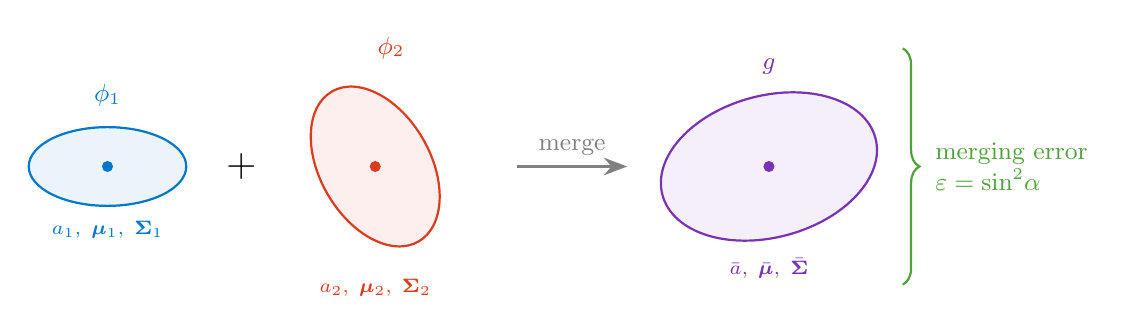
\begin{tikzpicture}[>=Stealth, scale=1.0]
  % ── Splat 1 ──
  \begin{scope}[shift={(-4.2,0)}]
    \draw[splat1, thick, fill=splat1!8]
      (0,0) ellipse (1.0 and 0.5);
    \fill[splat1] (0,0) circle (2pt);
    \node[splat1, above=4pt, font=\small\bfseries] at (0,0.5) {$\phi_1$};
    \node[splat1, below=2pt, font=\scriptsize] at (0,-0.5)
      {$a_1,\;\bmu_1,\;\Sig_1$};
  \end{scope}
  % ── Plus sign ──
  \node[font=\Large] at (-2.5,0) {$+$};
  % ── Splat 2 ──
  \begin{scope}[shift={(-0.8,0)}]
    \draw[splat2, thick, fill=splat2!8, rotate=30]
      (0,0) ellipse (0.7 and 1.1);
    \fill[splat2] (0,0) circle (2pt);
    \node[splat2, above=4pt, font=\small\bfseries] at (0.2,1.1)
      {$\phi_2$};
    \node[splat2, below=6pt, font=\scriptsize] at (0,-1.1)
      {$a_2,\;\bmu_2,\;\Sig_2$};
  \end{scope}
  % ── Arrow ──
  \draw[->, very thick, gray] (1.0, 0) -- node[above, font=\small]
    {merge} (2.4, 0);
  % ── Merged splat ──
  \begin{scope}[shift={(4.2,0)}]
    \draw[merged, thick, fill=merged!8, rotate=15]
      (0,0) ellipse (1.4 and 0.9);
    \fill[merged] (0,0) circle (2pt);
    \node[merged, above=4pt, font=\small\bfseries] at (0,0.9) {$g$};
    \node[merged, below=4pt, font=\scriptsize] at (0,-0.9)
      {$\bar a,\;\bar\bmu,\;\Sigbar$};
  \end{scope}
  % ── Error annotation ──
  \draw[decorate, decoration={brace, amplitude=6pt, mirror},
        residual, thick]
    (5.9, -1.5) -- (5.9, 1.5)
    node[midway, right=8pt, font=\small, residual, align=left]
    {merging error\\$\varepsilon = \sin^2\!\alpha$};
\end{tikzpicture}
\caption{Schematic of the merging operation.  Two oriented Gaussian
  splats $\phi_1$ and $\phi_2$ are replaced by a single splat~$g$.
  The merging error~$\varepsilon$ quantifies the fraction of the
  mixture's energy that cannot be captured by any single Gaussian.}
\label{fig:merge_schematic}
\end{figure}

\paragraph{Why \texorpdfstring{$L^2$}{L2}?}
To quantify how well a single Gaussian approximates a mixture, we
need a \emph{divergence}---a way to measure the ``distance'' between
two functions.  Several options exist (\cref{tab:divergences}), but
the $L^2$ (integrated squared error) framework is uniquely suited
because \emph{the integral of a product of two Gaussians has a
closed-form expression}.  Every term in the
error expansion reduces to such a product, yielding a fully analytical
result.  By contrast, the Kullback--Leibler divergence for a Gaussian
mixture involves $\log(\phi_1 + \phi_2)$, which has no closed form
\citep{hershey2007}; the Hellinger distance requires
$\sqrt{\phi_1 + \phi_2}$, equally intractable; and while the
2-Wasserstein distance between two individual Gaussians is elegant
\citep{jian2011}, it does not directly yield the error of
approximating a \emph{mixture}.

\begin{table}[ht]
\centering\small
\caption{Comparison of divergence measures for the merging problem.
  ``Mixture error'' refers to computing
  $d({\phi_1{+}\phi_2},\;g)$ analytically.}
\label{tab:divergences}
\begin{tabular}{@{}lccc@{}}
\toprule
\textbf{Divergence} & \textbf{Between two Gaussians} &
  \textbf{Mixture error} & \textbf{Optimal $g$} \\
\midrule
$L^2$ (ISE) & Closed-form & \textbf{Closed-form} & Numerical$^\dagger$ \\
KL & Closed-form & No closed-form & Moment-matched$^\ddagger$ \\
Hellinger & Closed-form & No closed-form & No closed-form \\
$W_2$ (Wasserstein) & Closed-form & No closed-form & Bures barycenter \\
\bottomrule
\end{tabular}

\vspace{4pt}
\raggedright\scriptsize
$^\dagger$\,Amplitude is closed-form; centre and covariance
require a few Newton iterations.\\
$^\ddagger$\,Minimises $\mathrm{KL}(f\|g)$ but the KL value itself
has no closed form.
\end{table}

\paragraph{Outline.}
\Cref{sec:kernel} derives the Gaussian $L^2$ inner product.
\Cref{sec:moment_match} constructs the moment-matched single-Gaussian
approximation.  \Cref{sec:error} states the closed-form error and the
$\sin^2\!\alpha$ mergeability score.  \Cref{sec:cosine} introduces a
cheaper ranking proxy.  \Cref{sec:special} treats important special
cases.  \Cref{sec:algorithm} provides pseudocode.
\Cref{sec:discussion} discusses optimality and practical
considerations.


% ══════════════════════════════════════════════════════════════════
\section{The Gaussian \texorpdfstring{$L^2$}{L2} Inner Product}\label{sec:kernel}
% ══════════════════════════════════════════════════════════════════

\subsection{Setup and Notation}

We work in $\R^D$.  A \textbf{Gaussian splat} is a function
\begin{equation}\label{eq:splat_def}
  \phi(\bx) \;=\; a \,\exp\!\Bigl(
    -\tfrac{1}{2}\,(\bx - \bmu)^\top \Sig^{-1} (\bx - \bmu)
  \Bigr),
  \qquad a > 0,\;\; \bmu \in \R^D,\;\;
  \Sig \succ 0
\end{equation}
where $\Sig \succ 0$ means $\Sig$ is symmetric positive definite
(i.e., it defines a valid ellipsoidal shape).
The covariance is stored via its \textbf{Cholesky factor}
$\Lchol$---a lower-triangular matrix satisfying
$\Sig = \Lchol\Lchol^\top$ (analogous to taking the ``square root''
of $\Sig$).  We also write $\Prec = \Sig^{-1}$ for the
\textbf{precision matrix} (the inverse covariance, which appears
naturally in the Gaussian exponent).  In the Luxar implementation,
$\Lchol$ is stored in packed row-major lower-triangular format with
$D(D{+}1)/2$ elements.

The \textbf{$L^2$ inner product} and norm used throughout are
\begin{equation}\label{eq:l2_ip}
  \langle f, g \rangle_{L^2}
  = \int_{\R^D} f(\bx)\,g(\bx)\,d\bx,
  \qquad
  \|f\|_{L^2}^2 = \langle f, f \rangle_{L^2}.
\end{equation}
Since $a > 0$ and $\Sig \succ 0$, every splat has finite energy
$\|\phi\|^2 < \infty$ and all inner products below are well-defined.

\subsection{Derivation of the Kernel}

The inner product $\langle\phi_i, \phi_j\rangle$ measures the
\emph{geometric overlap} between two Gaussians: it is large when
they sit close together with similar shapes, and vanishes when they
are far apart or oriented very differently.  The central result of
this section is that this overlap has a remarkably simple
closed-form expression.

\begin{theorem}[Gaussian $L^2$ inner product]\label{thm:kernel}
For two splats $\phi_i$, $\phi_j$ as in~\eqref{eq:splat_def},
\begin{equation}\label{eq:kernel}
\boxed{
  \langle \phi_i, \phi_j \rangle_{L^2}
  \;=\; a_i\,a_j \;(2\pi)^{D/2}\;
  \frac{\sqrt{|\Sig_i|\,|\Sig_j|}}
       {\sqrt{|\Sig_i + \Sig_j|}}\;
  \exp\!\Bigl(
    -\tfrac{1}{2}\,\Delta\bmu_{ij}^\top
    (\Sig_i + \Sig_j)^{-1}\,\Delta\bmu_{ij}
  \Bigr)
}
\end{equation}
where $\Delta\bmu_{ij} = \bmu_i - \bmu_j$.
\end{theorem}

\begin{proof}
Write the product of the two Gaussian kernels:
\begin{equation}\label{eq:product}
  \phi_i(\bx)\,\phi_j(\bx)
  = a_i a_j \exp\!\bigl(-\tfrac{1}{2}(Q_i + Q_j)\bigr),
\end{equation}
where $Q_k = (\bx - \bmu_k)^\top \Sig_k^{-1}(\bx - \bmu_k)$.
The sum of quadratic forms is itself quadratic in~$\bx$:
\begin{equation}\label{eq:sum_quad}
  Q_i + Q_j
  = \bx^\top \underbrace{(\Sig_i^{-1} + \Sig_j^{-1})}_{\displaystyle\Prec_{ij}} \bx
  - 2\,\bx^\top \underbrace{(\Sig_i^{-1}\bmu_i + \Sig_j^{-1}\bmu_j)}_{\displaystyle\bm{\eta}}
  + \underbrace{\bmu_i^\top\Sig_i^{-1}\bmu_i + \bmu_j^\top\Sig_j^{-1}\bmu_j}_{\displaystyle c}.
\end{equation}
Completing the square:
\begin{equation}\label{eq:complete_square}
  Q_i + Q_j
  = (\bx - \bmu_{ij})^\top \Prec_{ij}\,(\bx - \bmu_{ij})
  + \bigl(c - \bm{\eta}^\top \Prec_{ij}^{-1}\,\bm{\eta}\bigr),
\end{equation}
where $\bmu_{ij} = \Prec_{ij}^{-1}\bm{\eta}$ is the ``merged mean''
in precision space.  Integrating the Gaussian part over $\R^D$:
\begin{equation}
  \int_{\R^D}
    \exp\!\bigl(-\tfrac{1}{2}(\bx - \bmu_{ij})^\top\Prec_{ij}\,(\bx - \bmu_{ij})\bigr)
  \,d\bx
  = (2\pi)^{D/2}\,|\Prec_{ij}^{-1}|^{1/2}
  = \frac{(2\pi)^{D/2}}{|\Prec_{ij}|^{1/2}}.
\end{equation}
It remains to simplify the constant $c - \bm{\eta}^\top\Prec_{ij}^{-1}\bm{\eta}$.
Using the identity (see \cref{lem:identity}):
\begin{equation}\label{eq:constant_simplify}
  c - \bm{\eta}^\top \Prec_{ij}^{-1}\bm{\eta}
  = \Delta\bmu_{ij}^\top\;
    \Sig_i^{-1}\,\Prec_{ij}^{-1}\,\Sig_j^{-1}
    \;\Delta\bmu_{ij}
  = \Delta\bmu_{ij}^\top\;
    (\Sig_i + \Sig_j)^{-1}
    \;\Delta\bmu_{ij},
\end{equation}
and the determinant (using the harmonic-mean identity
$(\Sig_i^{-1}{+}\Sig_j^{-1})^{-1} = \Sig_i(\Sig_i{+}\Sig_j)^{-1}\Sig_j$,
which follows from \cref{lem:identity} by taking the inverse of both
sides of~\eqref{eq:matrix_identity} after multiplying by
$\Sig_i$ and $\Sig_j$):
\begin{equation}\label{eq:det_identity}
  |\Prec_{ij}^{-1}|
  = |(\Sig_i^{-1} + \Sig_j^{-1})^{-1}|
  = |\Sig_i(\Sig_i + \Sig_j)^{-1}\Sig_j|
  = \frac{|\Sig_i|\,|\Sig_j|}{|\Sig_i + \Sig_j|}.
\end{equation}
Combining: the integral of~\eqref{eq:product} factors as
$(2\pi)^{D/2}\,|\Prec_{ij}^{-1}|^{1/2}$ from~\eqref{eq:complete_square}
times $\exp(-\frac{1}{2}\cdot\text{\eqref{eq:constant_simplify}})$.
Rewriting $|\Prec_{ij}^{-1}|$ via~\eqref{eq:det_identity}
yields~\eqref{eq:kernel}.
\end{proof}

\begin{lemma}\label{lem:identity}
For symmetric positive definite $\Sig_i, \Sig_j$:
\begin{equation}\label{eq:matrix_identity}
  \Sig_i^{-1}(\Sig_i^{-1} + \Sig_j^{-1})^{-1}\Sig_j^{-1}
  = (\Sig_i + \Sig_j)^{-1}.
\end{equation}
\end{lemma}
\begin{proof}
Multiply both sides on the left by~$\Sig_i$ and on the right
by~$\Sig_j$.  The left side becomes
$(\Sig_i^{-1} + \Sig_j^{-1})^{-1}$ and the right side becomes
$\Sig_i(\Sig_i + \Sig_j)^{-1}\Sig_j$.  Taking the inverse of both sides:
$\Sig_i^{-1} + \Sig_j^{-1}$
versus
$\Sig_j^{-1}(\Sig_i + \Sig_j)\Sig_i^{-1}
 = \Sig_j^{-1} + \Sig_i^{-1}$.
These are equal since matrix addition commutes.
\end{proof}

\begin{figure}[ht]
\centering
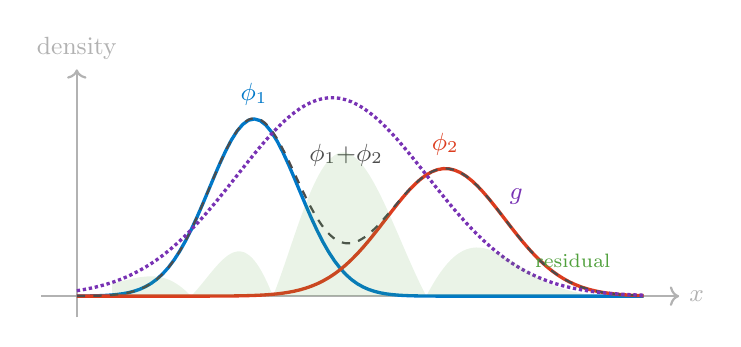
\begin{tikzpicture}[scale=0.9]
  % Axes
  \draw[->, thick, gray!60] (-0.5, 0) -- (8.5, 0)
    node[right, font=\small] {$x$};
  \draw[->, thick, gray!60] (0, -0.3) -- (0, 3.2)
    node[above, font=\small] {density};

  % Phi_1
  \draw[splat1, very thick, samples=100, domain=0:8]
    plot (\x, {2.5*exp(-0.5*(\x-2.5)^2/0.4)});
  \node[splat1, font=\small\bfseries] at (2.5, 2.85) {$\phi_1$};

  % Phi_2
  \draw[splat2, very thick, samples=100, domain=0:8]
    plot (\x, {1.8*exp(-0.5*(\x-5.2)^2/0.7)});
  \node[splat2, font=\small\bfseries] at (5.2, 2.15) {$\phi_2$};

  % Mixture (sum)
  \draw[black!70, thick, dashed, samples=200, domain=0:8]
    plot (\x, {2.5*exp(-0.5*(\x-2.5)^2/0.4) +
               1.8*exp(-0.5*(\x-5.2)^2/0.7)});
  \node[black!70, font=\small, above] at (3.8, 1.7) {$\phi_1{+}\phi_2$};

  % Merged Gaussian g
  \draw[merged, very thick, densely dotted, samples=100, domain=0:8]
    plot (\x, {2.8*exp(-0.5*(\x-3.6)^2/1.8)});
  \node[merged, font=\small\bfseries] at (6.2, 1.4) {$g$};

  % Residual shading (schematic)
  \fill[residual, opacity=0.12, samples=200, domain=0.5:7.5]
    plot (\x, {abs(2.5*exp(-0.5*(\x-2.5)^2/0.4) +
               1.8*exp(-0.5*(\x-5.2)^2/0.7) -
               2.8*exp(-0.5*(\x-3.6)^2/1.8))})
    -- (7.5, 0) -- (0.5, 0) -- cycle;
  \node[residual, font=\scriptsize] at (7.0, 0.5)
    {residual};
\end{tikzpicture}
\caption{One-dimensional illustration.  The mixture
  $\phi_1 + \phi_2$ (dashed) cannot be exactly represented by a single
  Gaussian~$g$ (dotted).  The shaded area (schematic) represents the
  residual whose squared integral is the merging error~$E$.}
\label{fig:1d_illustration}
\end{figure}

\begin{corollary}[Self inner product]\label{cor:self}
Setting $i = j$ and using $|2\Sig| = 2^D\,|\Sig|$:
\begin{equation}\label{eq:self_product}
  \|\phi_i\|^2_{L^2}
  = a_i^2\;\pi^{D/2}\;|\Sig_i|^{1/2}.
\end{equation}
\end{corollary}

\begin{remark}[In terms of Cholesky factors]
Since $\Sig_i = \Lchol_i\Lchol_i^\top$, we have
$|\Sig_i|^{1/2} = |\det \Lchol_i| = \prod_{k=1}^{D}(\Lchol_i)_{kk}$.
To evaluate the kernel~\eqref{eq:kernel}, form
$\bm{S} = \Sig_1 + \Sig_2 = \Lchol_1\Lchol_1^\top + \Lchol_2\Lchol_2^\top$,
compute $\bm{R} = \chol(\bm{S})$, and then
$|\Sig_1 + \Sig_2|^{1/2} = \prod_k \bm{R}_{kk}$.
The Mahalanobis term $(\Sig_1{+}\Sig_2)^{-1}\Delta\bmu$
is obtained by forward--backward substitution with~$\bm{R}$,
avoiding explicit matrix inversion.
\end{remark}


% ══════════════════════════════════════════════════════════════════
\section{The Moment-Matched Approximation}\label{sec:moment_match}
% ══════════════════════════════════════════════════════════════════

Armed with the closed-form kernel from \cref{sec:kernel}, we can now
construct the best single-Gaussian replacement for a pair of splats
and compute the resulting error analytically.

Given two splats $\phi_1, \phi_2$, we seek a single splat
$g(\bx) = \bar{a}\,\bar{G}(\bx)$
that best approximates their sum $f = \phi_1 + \phi_2$.
Throughout, we write $G_i(\bx) = \exp(-\frac{1}{2}(\bx - \bmu_i)^\top
\Sig_i^{-1}(\bx - \bmu_i))$ for the \textbf{unit-amplitude kernel}
of splat~$i$, so that $\phi_i = a_i\,G_i$.  Similarly,
$\bar{G}(\bx) = \exp(-\frac{1}{2}(\bx - \bar\bmu)^\top
\Sigbar^{-1}(\bx - \bar\bmu))$ denotes the unit-amplitude template
for the merged splat.

\subsection{Why Moment-Matching?}

Any density function can be summarised by its \emph{moments}: the
total mass (zeroth moment), the mean position (first moment), and the
spread or covariance (second moment).  A single Gaussian is fully
determined by its mean and covariance, so matching these moments is
the most natural way to ``compress'' a mixture into one Gaussian.

This intuition has a rigorous justification.  The Gaussian family
forms an \emph{exponential family} whose sufficient statistics are
$\bx$ and $\bx\bx^\top$ \citep{bishop2006}, and a classical result
from information geometry guarantees that the minimiser of the
Kullback--Leibler (KL) divergence from a target distribution to a
single Gaussian matches the target's mean and
covariance~\citep{bishop2006, west1993}.

Applied to our problem: we first normalise $f = \phi_1 + \phi_2$ to
a probability distribution, find the Gaussian whose mean and
covariance match (determining $\bar\bmu$ and $\Sigbar$), and then
set the amplitude $\bar{a}$ separately---either by mass conservation
(\cref{ssec:closed_form_params}) or by $L^2$ optimisation
(\cref{ssec:amp_opt}).  The moment-matched Gaussian is therefore the
canonical choice for single-component approximation.  Its shape
parameters have fully closed-form expressions.

\subsection{Closed-Form Parameters}\label{ssec:closed_form_params}

Define the \textbf{mass} of each splat and the mass-based weights:
\begin{equation}\label{eq:mass}
  m_i = a_i\,(2\pi)^{D/2}\,|\Sig_i|^{1/2}
  = \int_{\R^D} \phi_i(\bx)\,d\bx,
  \qquad
  w_i = \frac{m_i}{m_1 + m_2}.
\end{equation}

\begin{proposition}[Moment-matched parameters]\label{prop:mm}
The moment-matched single Gaussian $g$ has parameters:
\begin{align}
  \bar\bmu &= w_1\,\bmu_1 + w_2\,\bmu_2,
  \label{eq:mm_mean}\\[4pt]
  \Sigbar &= w_1\,\Sig_1 + w_2\,\Sig_2
    + w_1 w_2\,\Delta\bmu\,\Delta\bmu^\top,
  \label{eq:mm_cov}\\[4pt]
  \bar{a} &= \frac{m_1 + m_2}{(2\pi)^{D/2}\,|\Sigbar|^{1/2}}
    = \frac{a_1|\Sig_1|^{1/2} + a_2|\Sig_2|^{1/2}}{|\Sigbar|^{1/2}},
  \label{eq:mm_amp}
\end{align}
where $\Delta\bmu = \bmu_1 - \bmu_2$.
\end{proposition}

\begin{proof}
Treat the mixture as an unnormalised density with total mass
$M = m_1 + m_2$.  Normalising:
$p(\bx) = w_1\,\mathcal{N}(\bx;\bmu_1,\Sig_1)
  + w_2\,\mathcal{N}(\bx;\bmu_2,\Sig_2)$.
The mean is $\bar\bmu = w_1\bmu_1 + w_2\bmu_2$ by linearity.
The covariance uses the law of total variance:
\begin{equation}
  \Sigbar = \sum_i w_i\,\Sig_i
    + \sum_i w_i(\bmu_i - \bar\bmu)(\bmu_i - \bar\bmu)^\top.
\end{equation}
Substituting $\bmu_i - \bar\bmu = w_j\,(\bmu_i - \bmu_j)$
(where $j \neq i$) and $w_1 w_2^2 + w_2 w_1^2 = w_1 w_2$
yields~\eqref{eq:mm_cov}.  The amplitude~\eqref{eq:mm_amp} enforces
mass conservation $\int g = M$.
\end{proof}

\begin{figure}[ht]
\centering
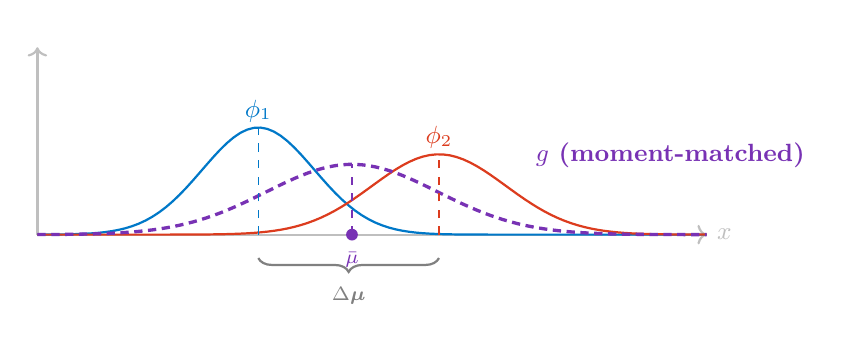
\begin{tikzpicture}[scale=0.85]
  \def\muA{-1.2}   \def\sigA{0.7}   \def\ampA{1.6}
  \def\muB{1.5}    \def\sigB{1.0}   \def\ampB{1.2}
  % Weights: wA = ampA*sigA / (ampA*sigA + ampB*sigB)
  %   = 1.12 / (1.12 + 1.2) = 0.483
  %   wB = 0.517
  \def\muM{0.2}    % weighted mean
  \def\sigM{1.65}  % moment-matched sigma^2 (approx)
  \def\ampM{1.05}  % mass-preserving amplitude (approx)

  % Axes
  \draw[->, thick, gray!50] (-4.5, 0) -- (5.5, 0)
    node[right, font=\small] {$x$};
  \draw[->, thick, gray!50] (-4.5, 0) -- (-4.5, 2.8)
    node[above, font=\small] {};

  % Individual splats
  \draw[splat1, thick, samples=100, domain=-4.5:5.5]
    plot (\x, {\ampA*exp(-0.5*(\x-\muA)^2/\sigA)});
  \node[splat1, font=\small\bfseries] at (\muA, \ampA+0.25) {$\phi_1$};

  \draw[splat2, thick, samples=100, domain=-4.5:5.5]
    plot (\x, {\ampB*exp(-0.5*(\x-\muB)^2/\sigB)});
  \node[splat2, font=\small\bfseries] at (\muB, \ampB+0.25) {$\phi_2$};

  % Moment-matched Gaussian
  \draw[merged, very thick, densely dashed, samples=100, domain=-4.5:5.5]
    plot (\x, {\ampM*exp(-0.5*(\x-\muM)^2/\sigM)});
  \node[merged, font=\small\bfseries, above right] at (2.8, 0.85)
    {$g$ (moment-matched)};

  % Mark means
  \draw[splat1, thin, dashed] (\muA, 0) -- (\muA, \ampA);
  \draw[splat2, thin, dashed] (\muB, 0) -- (\muB, \ampB);
  \draw[merged, thin, dashed] (\muM, 0) -- (\muM, \ampM);

  % Mark weighted mean
  \fill[merged] (\muM, 0) circle (2.5pt);
  \node[merged, below=3pt, font=\scriptsize] at (\muM, 0)
    {$\bar\mu$};

  % Brace for Delta mu
  \draw[decorate, decoration={brace, amplitude=5pt, mirror},
        gray, thick]
    (\muA, -0.35) -- (\muB, -0.35)
    node[midway, below=7pt, font=\scriptsize, gray]
    {$\Delta\bmu$};
\end{tikzpicture}
\caption{The moment-matched Gaussian $g$ (purple dashed) has its mean
  $\bar\bmu$ at the mass-weighted average of the two centres, and its
  covariance includes a rank-1 ``spreading'' term
  $w_1 w_2\,\Delta\bmu\,\Delta\bmu^\top$ due to the separation.}
\label{fig:moment_match}
\end{figure}

\begin{remark}[Geometric interpretation of $\Sigbar$]\label{rem:cov_decomp}
The moment-matched covariance decomposes as
$\Sigbar = \Sigbar_{\mathrm{intra}} + \Sigbar_{\mathrm{inter}}$,
where
$\Sigbar_{\mathrm{intra}} = w_1\Sig_1 + w_2\Sig_2$
is the weighted average of the individual spreads (the ``intrinsic''
width), and
$\Sigbar_{\mathrm{inter}} = w_1 w_2\,\Delta\bmu\,\Delta\bmu^\top$
is a rank-1 term encoding the ``extrinsic'' spread from the
separation of the two centres.  When $\bmu_1 = \bmu_2$, the extrinsic
term vanishes.
\end{remark}


% ══════════════════════════════════════════════════════════════════
\section{The Closed-Form Merging Error}\label{sec:error}
% ══════════════════════════════════════════════════════════════════

\subsection{Error Decomposition}

For \emph{any} single-Gaussian approximation~$g$, the $L^2$ error is:
\begin{equation}\label{eq:error_full}
  E = \|\phi_1 + \phi_2 - g\|^2_{L^2}
  = \underbrace{K_{11} + 2\,K_{12} + K_{22}}_{\displaystyle\|f\|^2}
    \;-\; 2\,K_{1g} - 2\,K_{2g} + K_{gg},
\end{equation}
where $K_{ij} = \langle\phi_i, \phi_j\rangle_{L^2}$ and
all six terms use the kernel from \cref{thm:kernel}.

\subsection{Amplitude Optimisation}\label{ssec:amp_opt}

The moment-matched amplitude~$\bar{a}$ from~\eqref{eq:mm_amp}
preserves the total mass, but is it the best choice for minimising
the $L^2$ error?  Not necessarily.  Since the shape parameters
$(\bar\bmu, \Sigbar)$ are already fixed, we can treat the amplitude
as a free knob and choose it optimally.

Rather than using the mass-preserving amplitude~$\bar{a}$
from~\eqref{eq:mm_amp}, we fix the moment-matched shape parameters
$(\bar\bmu, \Sigbar)$ and choose the amplitude that minimises the
$L^2$ error.  Write $\bar{G}(\bx) = \exp(-\frac{1}{2}(\bx {-}
\bar\bmu)^\top\Sigbar^{-1}(\bx {-} \bar\bmu))$ for the
unit-amplitude template.  Since
$E = \|f\|^2 - 2\bar{a}\,\langle f, \bar{G}\rangle + \bar{a}^2\,
\|\bar{G}\|^2$
is quadratic in~$\bar{a}$, the minimiser is
\begin{equation}\label{eq:a_star}
  a^* = \frac{\langle f, \bar{G} \rangle}{\|\bar{G}\|^2}
  = \frac{a_1\langle G_1, \bar{G}\rangle
    + a_2\langle G_2, \bar{G}\rangle}
    {\pi^{D/2}\,|\Sigbar|^{1/2}},
\end{equation}
and the corresponding minimum error is the classical
\textbf{projection residual}:
\begin{equation}\label{eq:E_star}
\boxed{
  E^* = \|f\|^2
  - \frac{\bigl|\langle f, \bar{G}\rangle\bigr|^2}{\|\bar{G}\|^2}
}
\end{equation}

This is strictly better than (or equal to) the mass-preserving
error, and still fully closed-form.

\subsection{The Mergeability Score}\label{ssec:mergeability}

The error~$E^*$ has units of ``energy squared,'' which depends on
the amplitudes and dimension.  To obtain a universal, dimensionless
measure, we normalise by the mixture's total energy~$\|f\|^2$.
The result has a beautiful geometric interpretation
(\cref{fig:angle_diagram}): think of the mixture~$f$ and the template
Gaussian~$\bar{G}$ as vectors in the infinite-dimensional Hilbert
space of square-integrable functions.  The best amplitude~$a^*$ is
the scalar projection of~$f$ onto~$\bar{G}$, exactly as in
ordinary Euclidean geometry, and the relative error is the sine
squared of the angle between them:

\begin{equation}\label{eq:mergeability}
\boxed{
  \varepsilon
  = \frac{E^*}{\|f\|^2}
  = 1 - \frac{\bigl|\langle f, \bar{G}\rangle\bigr|^2}
             {\|f\|^2\;\|\bar{G}\|^2}
  = 1 - \cos^2\!\alpha
  = \sin^2\!\alpha
}
\end{equation}
where $\alpha$ is the \textbf{angle between $f$ and $\bar{G}$ in
$L^2$} (the Hilbert space of square-integrable functions).

\begin{itemize}
\item $\varepsilon = 0$ ($\alpha = 0$): the two splats are
  proportional ($\phi_1 \propto \phi_2$), and the merge is perfect.
\item $\varepsilon \to 1$ ($\alpha \to \pi/2$): the mixture is
  nearly orthogonal to every single Gaussian with these shape
  parameters, and the merge is catastrophically lossy.
\end{itemize}

\begin{figure}[ht]
\centering
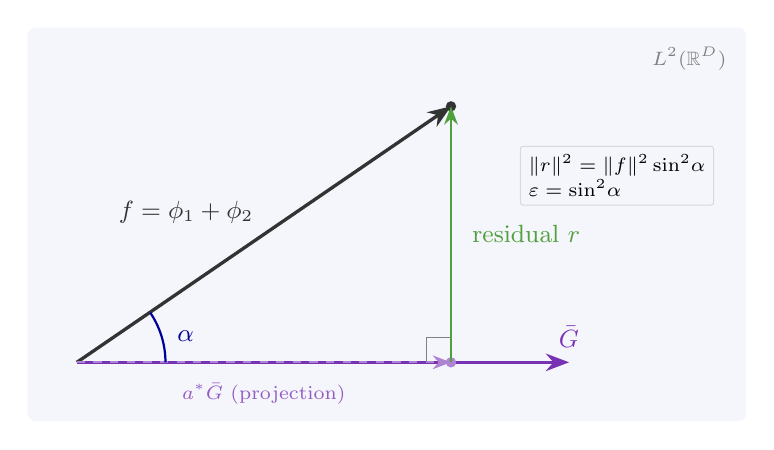
\begin{tikzpicture}[>=Stealth, scale=1.25]
  % coordinate system
  \coordinate (O) at (0,0);
  \coordinate (F) at (3.8, 2.6);
  \coordinate (Gproj) at (3.8, 0);
  \coordinate (Gdir) at (5.0, 0);

  % The L2 space axes (schematic)
  \fill[lightbg, rounded corners=3pt] (-0.5,-0.6) rectangle (6.8, 3.4);
  \node[gray, font=\scriptsize, anchor=north east] at (6.7, 3.3)
    {$L^2(\R^D)$};

  % Projection line
  \draw[gray, thin, dashed] (F) -- (Gproj);

  % f vector
  \draw[->, very thick, black!80] (O) -- (F)
    node[midway, above left, font=\small] {$f = \phi_1 + \phi_2$};
  \fill[black!80] (F) circle (1.5pt);

  % G direction arrow (full length, label ABOVE the arrow)
  \draw[->, very thick, merged] (O) -- (Gdir);
  \node[merged, font=\small, above=2pt] at (5.0, 0)
    {$\bar{G}$};

  % Projection (dashed, label BELOW the arrow near midpoint)
  \draw[->, thick, merged!60, dashed] (O) -- (Gproj);
  \fill[merged!60] (Gproj) circle (1.5pt);
  \node[merged!80, font=\scriptsize, below=4pt] at (1.9, 0)
    {$a^*\bar{G}$ (projection)};

  % Residual
  \draw[->, thick, residual] (Gproj) -- (F)
    node[midway, right=4pt, font=\small] {residual $r$};

  % Angle alpha
  \draw[thick, blue!60!black] (0.9, 0) arc (0:34:0.9)
    node[midway, right=2pt, font=\small] {$\alpha$};

  % Right angle mark
  \draw[gray, thin] (3.55, 0) -- (3.55, 0.25) -- (3.8, 0.25);

  % Annotations — use lightbg fill to match background
  \node[font=\scriptsize, align=left, anchor=north west,
        fill=lightbg, inner sep=3pt, rounded corners=1pt,
        draw=gray!30, thin]
    at (4.5, 2.2)
    {$\|r\|^2 = \|f\|^2\sin^2\!\alpha$\\[1pt]
     $\varepsilon = \sin^2\!\alpha$};
\end{tikzpicture}
\caption{Geometric interpretation in $L^2$.  The mixture
  $f = \phi_1 + \phi_2$ is a vector in the Hilbert space.  Its
  projection onto the ray spanned by~$\bar{G}$ (the unit-amplitude
  template) gives the optimal amplitude $a^*\bar{G}$.  The residual
  $r = f - a^*\bar{G}$ is orthogonal to~$\bar{G}$, and the normalised
  squared residual is $\varepsilon = \sin^2\!\alpha$.}
\label{fig:angle_diagram}
\end{figure}

\subsection{Expanding the Score}

For implementation, we expand the inner products in the mergeability
score into explicit kernel evaluations.  The score depends on four
types of kernel evaluation, listed in~\cref{tab:kernel_evals}.
Writing out all terms in~\eqref{eq:mergeability} using the
kernel~\eqref{eq:kernel}:

\begin{equation}\label{eq:score_expanded}
  \varepsilon = 1
  - \frac{\bigl(a_1\,I_1 + a_2\,I_2\bigr)^2}
         {\bigl(a_1^2\,J_1 + 2\,a_1 a_2\,I_{12} + a_2^2\,J_2\bigr)
          \;\cdot\; J_g}
\end{equation}
with the four kernel evaluations listed in \cref{tab:kernel_evals}.

\begin{table}[ht]
\centering\small
\caption{The four distinct kernel evaluations needed for the
  mergeability score.  All use the master formula~\eqref{eq:kernel}.}
\label{tab:kernel_evals}
\begin{tabular}{@{}cll@{}}
\toprule
\textbf{Symbol} & \textbf{Role} & \textbf{Expression} \\
\midrule
$J_i = \frac{\|\phi_i\|^2}{a_i^2}$
  & Self-energy (per unit $a_i^2$)
  & $\pi^{D/2}\,|\Sig_i|^{1/2}$ \\[6pt]
$J_g = \|\bar{G}\|^2$
  & Template self-energy
  & $\pi^{D/2}\,|\Sigbar|^{1/2}$ \\[6pt]
$I_{12} = \langle G_1, G_2 \rangle$
  & Cross-kernel (input splats)
  & $(2\pi)^{D/2}\,
    \dfrac{\sqrt{|\Sig_1|\,|\Sig_2\vphantom{|}|}}
          {\sqrt{|\Sig_1 + \Sig_2|}}
    \;e^{-Q_{12}/2}$ \\[10pt]
$I_i = \langle G_i, \bar{G}\rangle$
  & Cross-kernel (splat vs.\ template)
  & $(2\pi)^{D/2}\,
    \dfrac{\sqrt{|\Sig_i|\,|\Sigbar|}}
          {\sqrt{|\Sig_i + \Sigbar|}}
    \;e^{-\bar{Q}_i/2}$ \\[6pt]
\bottomrule
\end{tabular}

\vspace{6pt}
\raggedright\scriptsize
$Q_{12} = \Delta\bmu^\top(\Sig_1{+}\Sig_2)^{-1}\Delta\bmu$, \quad
$\bar{Q}_i = (\bar\bmu{-}\bmu_i)^\top(\Sig_i{+}\Sigbar)^{-1}(\bar\bmu{-}\bmu_i)$.
\end{table}


% ══════════════════════════════════════════════════════════════════
\section{Cheaper Proxy: The Inter-Splat Cosine}\label{sec:cosine}
% ══════════════════════════════════════════════════════════════════

Computing the full mergeability score requires four kernel evaluations
and forming the moment-matched covariance.  When the goal is merely to
\emph{rank} splat pairs by mergeability (e.g., to select the best
pair to merge next), a simpler proxy suffices:

\begin{proposition}[Inter-splat $L^2$ cosine]\label{prop:cosine}
The cosine similarity between two splats in $L^2$ is
amplitude-independent:
\begin{equation}\label{eq:cosine}
\boxed{
  \cos\theta
  = \frac{\langle\phi_1, \phi_2\rangle}
         {\|\phi_1\|\;\|\phi_2\|}
  = 2^{D/2}\;
    \frac{(|\Sig_1|\,|\Sig_2|)^{1/4}}
         {|\Sig_1 + \Sig_2|^{1/2}}\;
    \exp\!\bigl(-\tfrac{1}{2}\,Q_{12}\bigr)
}
\end{equation}
where $Q_{12} = \Delta\bmu^\top(\Sig_1 + \Sig_2)^{-1}\Delta\bmu$.
\end{proposition}

\begin{proof}
Direct computation from \eqref{eq:kernel} and \eqref{eq:self_product}:
the amplitudes $a_1, a_2$ cancel in the ratio, and
$(2\pi)^{D/2}/(\pi^{D/2})^{1/2 + 1/2} = 2^{D/2}$.
\end{proof}

\paragraph{Properties.}
\begin{itemize}
\item $\cos\theta = 1$ iff $\Sig_1 = \Sig_2$ and $\bmu_1 = \bmu_2$
  (identical shape and location).
\item $\cos\theta \to 0$ as $Q_{12} \to \infty$ (well-separated)
  or as the covariance shapes diverge.
\item Requires only \textbf{one} kernel evaluation (plus trivial
  self-products).
\item Strongly correlated with~$\varepsilon$ in practice, but does not
  account for amplitude ratios.  (By contrast, the full mergeability
  score~$\varepsilon$ depends on the ratio $a_1/a_2$ through $\|f\|^2$.)
\end{itemize}

\begin{remark}[Relationship between $\theta$ and $\alpha$]
The inter-splat angle~$\theta$ (between $\phi_1$ and $\phi_2$) and
the mergeability angle~$\alpha$ (between the mixture $f$ and
$\bar{G}$) are distinct quantities.  They agree in the extreme cases:
$\cos\theta = 1 \Leftrightarrow \varepsilon = 0$ (proportional
splats) and $\cos\theta = 0 \Rightarrow \varepsilon = 1$ (orthogonal
splats).  In between, the relationship is non-trivial because $\alpha$
depends on the moment-matched template~$\bar{G}$, while~$\theta$ is a
direct pairwise measure.  Nevertheless, $\cos\theta$ is an effective
proxy for ranking pairs by mergeability.
\end{remark}

\begin{figure}[ht]
\centering
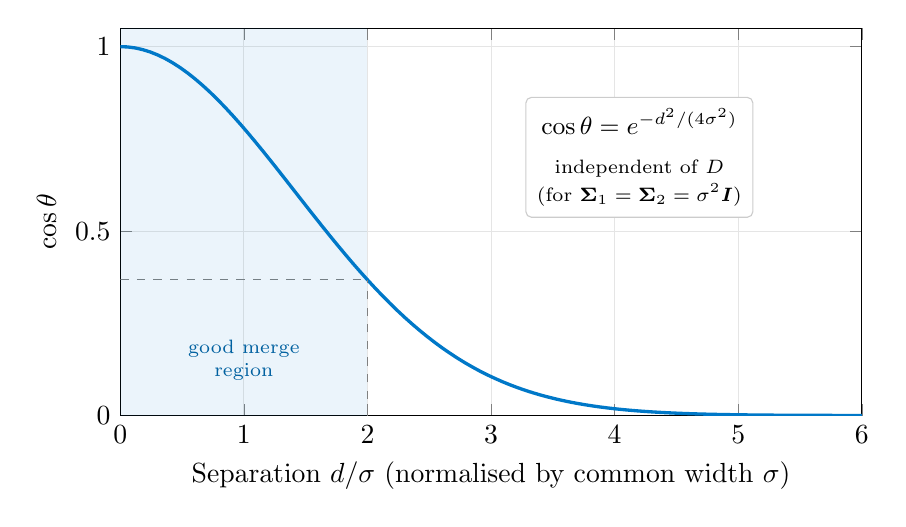
\begin{tikzpicture}
\begin{axis}[
  width=11cm, height=6.5cm,
  xlabel={Separation $d/\sigma$ (normalised by common width $\sigma$)},
  ylabel={$\cos\theta$},
  xmin=0, xmax=6, ymin=0, ymax=1.05,
  grid=major, grid style={gray!20},
  every axis plot/.append style={thick},
]

% For equal isotropic covariances: cos(theta) = exp(-d^2/(4*sigma^2)),
% independent of D.

\addplot[splat1, very thick, samples=100, domain=0:6]
  {exp(-x^2/4)};

% Threshold markers
\addplot[gray, dashed, thin, forget plot] coordinates {(2,0) (2,{exp(-1)})};
\addplot[gray, dashed, thin, forget plot] coordinates {(0,{exp(-1)}) (2,{exp(-1)})};
\node[font=\scriptsize, gray, anchor=east] at (axis cs:-0.05, {exp(-1)})
  {$e^{-1}\!\approx 0.37$};
\node[font=\scriptsize, gray, anchor=north] at (axis cs:2, -0.03)
  {$2\sigma$};

% Main annotation
\node[font=\small, align=center, fill=white, inner sep=4pt,
      draw=gray!40, rounded corners=2pt] at (axis cs:4.2, 0.7)
  {$\cos\theta = e^{-d^2/(4\sigma^2)}$\\[3pt]
   \scriptsize independent of $D$\\[-1pt]
   \scriptsize (for $\Sig_1 = \Sig_2 = \sigma^2\bm{I}$)};

% Practical zone
\fill[splat1, opacity=0.08] (axis cs:0,0) rectangle (axis cs:2, 1.05);
\node[font=\scriptsize, splat1!80!black, align=center] at (axis cs:1.0, 0.15)
  {good merge\\region};

\end{axis}
\end{tikzpicture}
\caption{Inter-splat cosine similarity vs.\ normalised separation
  for two splats with equal isotropic covariances
  $\Sig_1 = \Sig_2 = \sigma^2\bm{I}$.  The result
  $\cos\theta = \exp(-d^2/4\sigma^2)$ is independent of the
  dimension~$D$: the $2^{D/2}$ prefactor in~\eqref{eq:cosine}
  exactly cancels the determinant ratio for equal covariances.
  The shaded region ($d \lesssim 2\sigma$, $\cos\theta \gtrsim e^{-1}$)
  indicates practically mergeable pairs.}
\label{fig:cosine_vs_distance}
\end{figure}


% ══════════════════════════════════════════════════════════════════
\section{Special Cases}\label{sec:special}
% ══════════════════════════════════════════════════════════════════

To build intuition for the general formulas, we examine three
limiting cases where the expressions simplify dramatically and yield
practical rules of thumb.

\subsection{Equal Isotropic Covariances}
\label{ssec:iso}

When $\Sig_1 = \Sig_2 = \sigma^2\bm{I}_D$, the kernel simplifies
dramatically.  Let $d = \|\Delta\bmu\|$:
\begin{align}
  K_{12} &= a_1 a_2\,\pi^{D/2}\,\sigma^D\,
    e^{-d^2/(4\sigma^2)}, \label{eq:K12_iso}\\
  \|f\|^2 &= (a_1^2 + a_2^2)\,\pi^{D/2}\,\sigma^D
    + 2\,a_1 a_2\,\pi^{D/2}\,\sigma^D\,e^{-d^2/(4\sigma^2)},
    \label{eq:f_norm_iso}\\
  \cos\theta &= e^{-d^2/(4\sigma^2)}.
    \label{eq:cos_iso}
\end{align}
The dimension-dependence vanishes because the $2^{D/2}$ prefactor
in~\eqref{eq:cosine} exactly cancels the determinant ratio
$|\sigma^2\bm{I}|^{1/2}/|2\sigma^2\bm{I}|^{1/2} = 2^{-D/2}$
for equal covariances.
The inter-splat cosine thus depends only on the ratio $d/\sigma$,
offering a simple and intuitive merging criterion: merge when
$d \lesssim 2\sigma$ (where $\cos\theta \gtrsim e^{-1} \approx 0.37$).

\subsection{Co-located Splats (\texorpdfstring{$\bmu_1 = \bmu_2$}{mu1 = mu2})}
\label{ssec:colocated}

When the centres coincide, $Q_{12} = 0$ and
$\Sigbar_{\mathrm{inter}} = 0$, so:
\begin{equation}
  \cos\theta = 2^{D/2}\,
  \frac{(|\Sig_1|\,|\Sig_2|)^{1/4}}{|\Sig_1 + \Sig_2|^{1/2}}.
\end{equation}
This depends purely on the \emph{shape} discrepancy.  For isotropic
splats with $\Sig_i = \sigma_i^2\bm{I}$:
\begin{equation}
  \cos\theta = \frac{2^{D/2}\,(\sigma_1\sigma_2)^{D/2}}
    {(\sigma_1^2 + \sigma_2^2)^{D/2}}
  = \left(\frac{2\sigma_1\sigma_2}{\sigma_1^2 + \sigma_2^2}\right)^{D/2}
  = \left(\frac{2}{r + r^{-1}}\right)^{D/2},
\end{equation}
where $r = \sigma_1/\sigma_2$ is the width ratio.  This is the
geometric--harmonic mean ratio raised to the $D/2$ power.  It equals~1
when $r=1$ and decays rapidly as $r$ departs from unity, especially in
high dimensions (\cref{fig:colocated_cosine}).

\begin{figure}[ht]
\centering
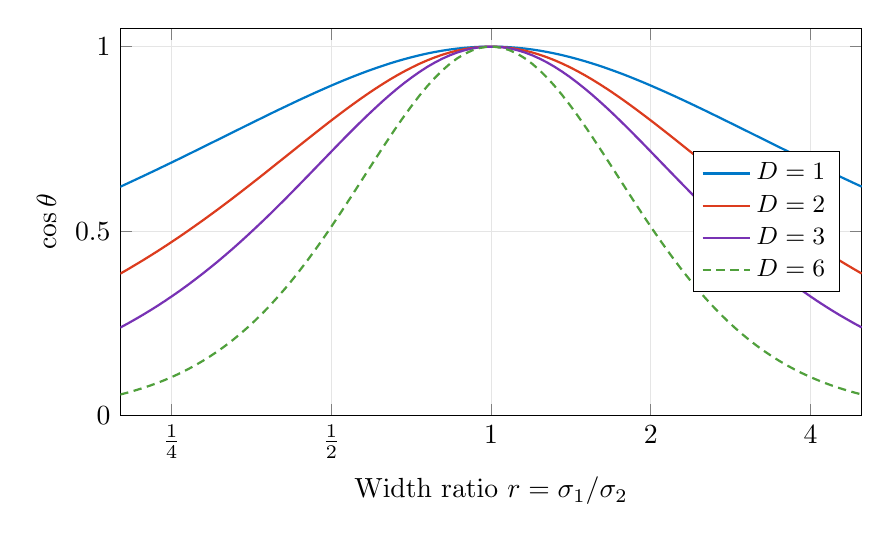
\begin{tikzpicture}
\begin{axis}[
  width=11cm, height=6.5cm,
  xlabel={Width ratio $r = \sigma_1 / \sigma_2$},
  ylabel={$\cos\theta$},
  xmin=0.2, xmax=5, ymin=0, ymax=1.05,
  grid=major, grid style={gray!20},
  legend style={at={(0.97,0.5)}, anchor=east, font=\small},
  every axis plot/.append style={thick},
  xmode=log, log basis x=2,
  xtick={0.25, 0.5, 1, 2, 4},
  xticklabels={$\frac{1}{4}$, $\frac{1}{2}$, $1$, $2$, $4$},
]

\addplot[splat1, samples=100, domain=0.2:5]
  {(2/(x + 1/x))^(0.5)};
\addlegendentry{$D = 1$}

\addplot[splat2, samples=100, domain=0.2:5]
  {(2/(x + 1/x))^(1)};
\addlegendentry{$D = 2$}

\addplot[merged, samples=100, domain=0.2:5]
  {(2/(x + 1/x))^(1.5)};
\addlegendentry{$D = 3$}

\addplot[residual, samples=100, domain=0.2:5, densely dashed]
  {(2/(x + 1/x))^(3)};
\addlegendentry{$D = 6$}

\end{axis}
\end{tikzpicture}
\caption{Inter-splat cosine for co-located isotropic splats as a
  function of the width ratio.  Higher dimensions penalise shape
  differences more severely: in $D=3$, a $2{\times}$ width ratio
  already drops the cosine to $\approx 0.60$.}
\label{fig:colocated_cosine}
\end{figure}

\subsection{Proportional Splats (\texorpdfstring{$\phi_1 \propto \phi_2$}{phi1 proportional to phi2})}
\label{ssec:proportional}

When $\bmu_1 = \bmu_2$ and $\Sig_1 = \Sig_2$, the two splats are
proportional: $\phi_1 + \phi_2 = (a_1 + a_2)\,G(\bx;\bmu,\Sig)$, which
is already a single Gaussian.  In this case $\cos\theta = 1$ and
$\varepsilon = 0$: the merge is exact.


% ══════════════════════════════════════════════════════════════════
\section{Algorithm}\label{sec:algorithm}
% ══════════════════════════════════════════════════════════════════

\Cref{alg:mergeability} computes the full mergeability score for
a pair of splats.  \Cref{alg:cosine} provides the cheaper cosine
proxy for ranking.  \Cref{alg:merge} constructs the merged splat
using either mass-preserving or $L^2$-optimal amplitude.

\clearpage
\begin{algorithm}[H]
\caption{Mergeability score for a pair of Gaussian splats}
\label{alg:mergeability}
\KwIn{Splats $(a_1, \bmu_1, \Lchol_1)$ and $(a_2, \bmu_2, \Lchol_2)$
  in $\R^D$}
\KwOut{Mergeability score $\varepsilon \in [0,1]$
  and optimal merged parameters $(\bar{a}, \bar\bmu, \Sigbar)$}
\BlankLine
\tcc{Step 1: Form covariances}
$\Sig_i \gets \Lchol_i\,\Lchol_i^\top$ for $i = 1,2$\;
\BlankLine
\tcc{Step 2: Moment-matched parameters}
$d_i \gets \prod_k (\Lchol_i)_{kk}$
  \tcp*{$|\Sig_i|^{1/2} = |\det \Lchol_i|$}
$m_i \gets a_i\,(2\pi)^{D/2}\,d_i$ \tcp*{mass}
$w_i \gets m_i\,/\,(m_1 + m_2)$\;
$\bar\bmu \gets w_1\,\bmu_1 + w_2\,\bmu_2$\;
$\Delta\bmu \gets \bmu_1 - \bmu_2$\;
$\Sigbar \gets w_1\,\Sig_1 + w_2\,\Sig_2
  + w_1 w_2\,\Delta\bmu\,\Delta\bmu^\top$\;
$\bar\Lchol \gets \chol(\Sigbar)$\;
$d_g \gets \prod_k \bar\Lchol_{kk}$ \tcp*{$|\Sigbar|^{1/2}$}
\BlankLine
\tcc{Step 3: Self-energies}
$J_i \gets \pi^{D/2}\,d_i$ for $i = 1,2$\;
$J_g \gets \pi^{D/2}\,d_g$\;
\BlankLine
\tcc{Step 4: Cross-kernels (input pair)}
$\bm{S}_{12} \gets \Sig_1 + \Sig_2$\;
$\bm{R}_{12} \gets \chol(\bm{S}_{12})$\;
$\bm{v} \gets$ solve $\bm{S}_{12}\,\bm{v} = \Delta\bmu$
  \tcp*{via $\bm{R}_{12}$}
$Q_{12} \gets \Delta\bmu^\top\bm{v}$\;
$d_{12} \gets \prod_k (\bm{R}_{12})_{kk}$\;
$I_{12} \gets (2\pi)^{D/2}\,(d_1\,d_2)\,/\,d_{12}
  \;\cdot\;\exp(-Q_{12}/2)$\;
\BlankLine
\tcc{Step 5: Cross-kernels (splat vs.\ template)}
\For{$i \in \{1, 2\}$}{
  $\bm{S}_i \gets \Sig_i + \Sigbar$\;
  $\bm{R}_i \gets \chol(\bm{S}_i)$\;
  $\bz \gets$ solve $\bm{S}_i\,\bz = \bar\bmu - \bmu_i$\;
  $\bar{Q}_i \gets (\bar\bmu - \bmu_i)^\top\bz$\;
  $I_i \gets (2\pi)^{D/2}\,(d_i\,d_g)\,/\,\prod_k(\bm{R}_i)_{kk}
    \;\cdot\;\exp(-\bar{Q}_i/2)$\;
}
\BlankLine
\tcc{Step 6: Mergeability score}
$\|f\|^2 \gets a_1^2\,J_1 + 2\,a_1 a_2\,I_{12} + a_2^2\,J_2$\;
$\langle f, \bar{G}\rangle \gets a_1\,I_1 + a_2\,I_2$\;
$\varepsilon \gets 1
  - \langle f, \bar{G}\rangle^2\,/\,(\|f\|^2 \cdot J_g)$\;
\BlankLine
\tcc{Step 7: $L^2$-optimal amplitude}
$\bar{a} \gets \langle f, \bar{G}\rangle\,/\,J_g$\;
\Return $\varepsilon$, $(\bar{a}, \bar\bmu, \Sigbar)$\;
\end{algorithm}


\begin{algorithm}[H]
\caption{Quick mergeability ranking via inter-splat cosine}
\label{alg:cosine}
\KwIn{Splats $(a_1, \bmu_1, \Lchol_1)$ and $(a_2, \bmu_2, \Lchol_2)$}
\KwOut{Cosine similarity $\cos\theta \in [0,1]$}
\BlankLine
$\Sig_i \gets \Lchol_i\,\Lchol_i^\top$ for $i = 1,2$\;
$\bm{S} \gets \Sig_1 + \Sig_2$\;
$\bm{R} \gets \chol(\bm{S})$\;
$\Delta\bmu \gets \bmu_1 - \bmu_2$\;
$\bw \gets$ solve $\bm{S}\,\bw = \Delta\bmu$\;
$Q \gets \Delta\bmu^\top \bw$\;
$\cos\theta \gets 2^{D/2}
  \cdot \dfrac{\bigl(\prod_k(\Lchol_1)_{kk}\bigr)^{1/2}
               \;\bigl(\prod_k(\Lchol_2)_{kk}\bigr)^{1/2}}
              {\prod_k(\bm{R})_{kk}}
  \cdot e^{-Q/2}$\;
\Return $\cos\theta$\;
\end{algorithm}

\begin{algorithm}[H]
\caption{Construct the merged splat}
\label{alg:merge}
\KwIn{Splats $(a_i, \bmu_i, \Lchol_i)$ for $i=1,2$; desired mode
  (\texttt{mass} or \texttt{L2})}
\KwOut{Merged splat $(\bar{a}, \bar\bmu, \bar\Lchol)$}
\BlankLine
Compute $\bar\bmu$, $\Sigbar$, $\bar\Lchol = \chol(\Sigbar)$
  as in \cref{alg:mergeability} Steps~1--2\;
\BlankLine
\uIf{\normalfont mode = \texttt{mass}}{
  $m_i \gets a_i\,(2\pi)^{D/2}\prod_k(\Lchol_i)_{kk}$ for $i=1,2$\;
  $\bar{a} \gets (m_1 + m_2)\,/\,\bigl((2\pi)^{D/2}
    \prod_k\bar\Lchol_{kk}\bigr)$
    \tcp*{mass-preserving}
}
\Else{
  Compute $I_1, I_2$ and $J_g$
    as in \cref{alg:mergeability} Steps~3--5\;
  $\bar{a} \gets (a_1 I_1 + a_2 I_2)\,/\,J_g$
    \tcp*{$L^2$-optimal}
}
\Return $(\bar{a}, \bar\bmu, \bar\Lchol)$\;
\end{algorithm}


% ══════════════════════════════════════════════════════════════════
\section{Optimality Discussion}\label{sec:discussion}
% ══════════════════════════════════════════════════════════════════

\subsection{Is This the True Minimum \texorpdfstring{$L^2$}{L2} Error?}

The mergeability score~$\varepsilon$ uses moment-matched
$\bar\bmu, \Sigbar$ with $L^2$-optimised amplitude.  The
\emph{globally} $L^2$-optimal Gaussian would also optimise
$\bar\bmu$ and $\Sigbar$, satisfying:
\begin{equation}\label{eq:stationarity}
  \sum_i a_i\,\lambda_i\,(\Sig_i + \Sigbar)^{-1}(\bar\bmu - \bmu_i) = 0,
\end{equation}
where $\lambda_i = \langle G_i, \bar{G}\rangle$ depends on
$\bar\bmu$ and $\Sigbar$---a nonlinear system with no general
closed-form solution.  Thus:

\begin{itemize}
\item The score~$\varepsilon$ is an \textbf{upper bound} on the true
  minimum relative $L^2$ error.
\item In practice, the moment-matched and $L^2$-optimal solutions
  are \textbf{very close} when the two covariances are similar
  (the typical case for merge candidates).
\item For exact minimisation when needed, a few iterations of
  Gauss--Newton starting from the moment-matched solution converge
  rapidly.
\item The error formula~\eqref{eq:error_full} is exact for
  \emph{any} choice of~$g$, so one can always evaluate the true
  $L^2$ error once the optimal parameters are found numerically.
\end{itemize}

\subsection{When Does Moment-Matching Equal \texorpdfstring{$L^2$}{L2}-Optimal?}

\begin{enumerate}
\item \textbf{Proportional splats}
  ($\phi_1 \propto \phi_2$): trivially, $\varepsilon = 0$ for
  both.
\item \textbf{Equal amplitudes and equal covariances}
  ($a_1 = a_2$, $\Sig_1 = \Sig_2$): by symmetry, the optimal
  mean is $(\bmu_1{+}\bmu_2)/2$, which is also the
  moment-matched mean.  The optimal covariance still differs
  from the moment-matched one in general, but the difference is
  typically small.
\end{enumerate}

\subsection{Relationship to Existing Merging Criteria}

\begin{itemize}
\item \textbf{Runnalls' KL bound}~\citep{runnalls2007}: an upper
  bound on the KL divergence cost of merging.  It is
  $B_{12} = \frac{1}{2}\bigl[(w_1{+}w_2)\log|\Sigbar|
  - w_1\log|\Sig_1| - w_2\log|\Sig_2|\bigr]$,
  which only measures the covariance mismatch and is blind to
  amplitude differences.  Our $L^2$ score incorporates amplitudes
  and the full geometric overlap.

\item \textbf{ISE-based reduction}~\citep{williams2003, scott2001}:
  uses $\|f - g\|^2_{L^2}$ directly, as we do.  Our contribution is
  the explicit factorisation into the $\sin^2\!\alpha$ form and the
  amplitude-optimised closed-form expression.

\item \textbf{Salmond's method}~\citep{salmond1990}: merges components
  with the smallest increase in ISE, equivalent to choosing the pair
  with the smallest~$E^*$.
\end{itemize}

\subsection{Practical Considerations}

\paragraph{Truncation.}
The Luxar implementation uses a shifted truncated Gaussian
$a \cdot s \cdot \max\!\bigl(0,\; e^{-\mathcal{M}^2/2} - C\bigr)$,
where $\mathcal{M}$ is the Mahalanobis distance,
$s = 1/(1{-}C)$ is a peak-preserving scale factor, and
$C = e^{-T^2/2} \approx 0.011$ for $T=3$.  The tails beyond
$T$ standard deviations contribute $< 1.2\%$ of the total energy,
so the pure-Gaussian analysis provides an excellent approximation.

\paragraph{Computational cost.}
For $D = 3$: three Cholesky factorisations of $3\times 3$ matrices,
three linear solves, and scalar arithmetic.  Total: $\sim 200$
floating-point operations per pair, negligible compared to the
rendering cost.

\paragraph{Batch processing.}
For culling, precompute $J_i = \pi^{D/2}\,|\det\Lchol_i|$ and
$m_i$ for all splats.  The per-pair cost then reduces to one
kernel evaluation $I_{12}$ (for the cosine proxy) or four kernel
evaluations (for the full score).


% ══════════════════════════════════════════════════════════════════
\section{Summary}\label{sec:summary}
% ══════════════════════════════════════════════════════════════════

\begin{enumerate}
\item The $L^2$ integrated squared error is the unique divergence
  for which \emph{all} terms in the Gaussian merging error have
  closed-form expressions.

\item The moment-matched Gaussian (KL-optimal) provides a
  closed-form approximation whose shape parameters are given
  by~\eqref{eq:mm_mean}--\eqref{eq:mm_cov}, with $L^2$-optimal
  amplitude from~\eqref{eq:a_star}.

\item The normalised merging error is
  $\varepsilon = \sin^2\!\alpha$ (\cref{eq:mergeability}),
  where $\alpha$ is the angle between the mixture and the template
  Gaussian in~$L^2$.

\item For ranking pairs cheaply, the inter-splat cosine
  (\cref{eq:cosine}) requires only one kernel evaluation and is
  amplitude-independent.

\item For equal isotropic covariances, the cosine reduces to
  $\exp(-d^2/4\sigma^2)$, depending only on the normalised
  separation.
\end{enumerate}


% ══════════════════════════════════════════════════════════════════
\bibliographystyle{plainnat}
\bibliography{references}
% ══════════════════════════════════════════════════════════════════

\end{document}
